\documentclass[12pt, letterpaper]{article}
\usepackage[utf8]{inputenc}
\usepackage[margin=1in]{geometry}
\usepackage{times}
\usepackage{hyperref}
\usepackage{graphicx}
\usepackage{gensymb}
\usepackage{caption}
\renewcommand{\abstractname}{\vspace{-\baselineskip}}

% Document
\begin{document}
\begin{center}
    \Large X-ray, Optical, and Radio Solar Event Identification and Prediction using Neural Networks \\
    \vspace{.6em}
    \large Ted Grosson, Cody Meng, Preston Tracy, Jackson White, Yiwen Zhu
    \vspace{.3em}
    \\ Advisor: Chris Tunnell | Rice University
    \vspace{.5em}
    \normalsize
    \\ Submitted February 22, 2021
    \\
    \vspace{1em}
    \textbf{Project Pitch} \end{center} \vspace{-2.3em}

\begin{abstract} \normalsize
Solar events, such as flares and prominences, can lead to detrimental effects on Earth systems by disrupting electronics and communication systems, particularly in satellites with limited protection from Earth’s magnetic field. Due to the potential harm of these events, it would be remarkably useful to identify and predict these events when or before they occur to allow rapid preparatory actions to mitigate potential damages as much as possible. We propose applying machine learning techniques to historical solar data from NASA’s Solar Dynamics Observatory in order to train a set of neural networks to identify and predict solar events from live multi-waveband imaging of the Sun. The Solar Dynamics Observatory (SDO) satellite was launched in 2010 and continuously observes the Sun on roughly 10-minute intervals with multiple imaging instruments. In particular, the Atmospheric Imaging Assembly (AIA) aboard SDO images the sun in wavelengths ranging from the UV to optical, providing a constant stream of live, high-resolution solar information \cite{Pesnell2012}. Using the images obtained from AIA, we should be able to easily identify x-ray and optical events and prominences emanating from the Sun. By analyzing historical AIA data prior to and during documented solar events, we may be able to construct a tool that predicts solar events before and as they actually occur.
\end{abstract}

\section*{Core Scientific Question}

In this project, we plan to identify and predict specific solar events from multi-waveband observations of the Sun obtained from the Solar Dynamics Observatory Atmospheric Imaging Assembly. The cause of solar flares and prominences are most often attributed to magnetic fields, but we lack a concrete mechanism by which such events take place \cite{BOB}. Determining whether visible precursors to solar events exist, how early they take place, and how prominently they appear in each waveband, may provide valuable constraints on the theoretical mechanisms by which these solar events are created. Even if we fail to produce a neural network capable of predicting solar events before they occur, this failure may indicate that solar events lack temporal precursors large or coherent enough to appear on the Sun’s surface in x-ray, ultraviolet, and optical wavelength images. Because we are applying similar methods to both identification and prediction of solar events, we can perform at least a cursory analysis comparing the efficacy of our tools applied to both problems, which could provide a point of comparison between the visibility of solar events precursors to the events themselves. 

We also hope to determine whether we can precisely identify solar radio events from optical or ultraviolet images of the Sun, as it is unclear as to the degree of precision by which we can identify solar events outside of their principal wavelengths. Should some solar events be recognizable in shorter wavelength images, we may be able to use this information to constrain or classify radio events. For example, if one type of radio event produces an identifiable signature in the optical while another does not, we may be able to use our tools to aid in classifying these events, providing additional clues as to the mechanisms by which either type of event can take place. In addition, if we are able to predict radio events in the optical or ultraviolet, this would provide similar benefits to those described in the previous paragraph: namely, determining how early, prominently, and in what wavelengths precursors to these events can occur. 

\section*{Project Objectives}

Our project objectives fall under three overarching steps, which we will discuss in detail within this section. 

First, we will attempt to train a neural network to identify solar events from solar images, using historical SDO AIA solar images in 5-6 wavebands between 90 and 300 Angstroms alongside solar event reports obtained from NOAA's Space Weather Prediction Center. The images and solar event reports will be aligned in time, so that the neural network will learn to associate features within the images with specific types of solar events. We will initially focus on two types of events, x-ray events and optical flares. 

Next, we will apply this same methodology to radio bursts. We will attempt to use the longest wavelengths available to us on the AIA, but radio emission is well outside of the low-frequency limit of the accessible bandpasses. That being said, we will still train a neural network on similar sets of AIA images alongside simultaneous radio burst reports. If radio bursts carry signature features present in higher-frequency wavebands, our neural network may be able to identify them. 

Finally, should the previous steps be successful, we will transition to prediction of solar events rather than identification. Our overall methodology is the same, but we will train our neural networks on solar event data alongside images taken at various time intervals before the solar events occurred. We will experiment with various time lags, training several neural networks on different lags simultaneously, and evaluating what time lags are optimal or effective for certain kinds of events. With an understanding of predictive accuracy as a function of time lag, we can determine whether and when notable surface signatures arise as precursors to x-ray, optical, and radio solar events. The previous two steps will both serve as points of comparison between the efficacy of our identification and prediction networks as well as provide a proof of concept demonstration of how our predictive network may function under ideal conditions, with a time lag of zero. 


\section*{Data Description}

\subsection*{AIA Observations}

In this project we will be using two primary datasets: Atmospheric Imaging Assembly (AIA) instrument observations of the sun, from the Solar Dynamics Observatory (SDO), and space weather reports from the National Oceanic and Atmospheric Administration (NOAA).
The AIA takes observations at ten different wavelengths, which are summarized in in Table \ref{AIA_wavelengths}, which each probe different layers of the sun. The AIA has been observing the sun since 2010, and observes at 4500 Å once every hour, at 1600 and 1700 Å once every 24 seconds, and at the remaining wavelengths once 12 seconds. The images are stored as 4096x4096 pixel .fits files, where each pixel represents the flux captured by the corresponding pixel on the AIA CCD. The headers of the .fits files also include relevant information such as the exposure time and time of the observation. These files can be queried and downloaded from within python, using the sunpy package. Using sunpy we can select images based on their observation time and filter, which will allow us to easily select and download observations which correspond to events in the space weather reports. 

The different wavelengths observed by AIA were chosen to examine a specific portion of the Sun’s surface or atmosphere. Each of these wavelengths are centered on a different emission line to examine the features visible at the temperature of the emission line. The EUV wavelengths observe extremely hot temperatures, and are centered on different iron ions, ranging from Fe IX (171 Å) to Fe XXIII (131 Å), and observing temperatures from 60,000 K (304 Å) to 20,000,000 K (193 Å) \cite{Lemen2012}. The 1700 Å and 4500 Å wavelengths show continuum images of the Sun in the UV and optical, respectively. The 1600 Å wavelength examines the transition region between the chromosphere and the corona. The 304 Å wavelength also examines the transition region, as well as the chromosphere. The 171 Å wavelength shows the “quiet” (low magnetic activity) corona and coronal loops, and the 193 Å examines a hotter region of the corona, as well as the hotter material in solar flares. The 211 Å and 335 Å wavelengths both examine the hot, magnetically active regions of the corona. Finally, the 94 Å and 131 Å wavelengths both examine flaring regions, with wavelengths centered at different temperatures \cite{Zell2015}. The temperature coverage provided by these wavelengths allows for a more complete reconstruction of thermal structure than previous missions \cite{AIA_ConceptReport}.

\begin{table}
\begin{center}
 \begin{tabular}{||c | c ||} 
 \hline
 Acronym & Full Name \\ [0.5ex] 
 \hline\hline
 BSL & Bright Surge on Limb \\
 \hline
 DSF & Filament Disappearance \\ 
 \hline
    EPL & Eruptive Prominence on Limb\\
 \hline
    FIL & Filament\\
 \hline
    FLA & Optical Flare in H-Alpha\\
 \hline
    FOR & Forbush Decrease (CR Decrease) \\
 \hline
    GLE & Ground-Level Event (CR Increase) \\
 \hline
    LPS & Loop Prominence System\\
 \hline
    PCA & Polar Cap Absorption\\
 \hline
    RBR & Fixed-Frequency Radio Burst\\
 \hline
    RNS & Radio Noise Storm\\
 \hline
    RSP & Sweep-Frequency Radio Burst\\
 \hline
    SPY & Spray\\
 \hline
    XRA & X-ray Event \\
 \hline
\end{tabular}
\caption{Events tracked in space weather reports}
\label{space_weather_events}
\end{center}
\end{table}

\subsection*{NOAA Space Weather Reports}

The second dataset, the space weather reports, are created once per day by the NOAA and can contain 13 different types of space weather events, which are listed in Table \ref{space_weather_events}. These reports exist back until 1997, so we have corresponding reports for all AIA data. A sample report from 2015 is depicted in Figure \ref{swr_sample}. The entire collection of reports amounts to only 18 MB in storage size, so we are able to store all the reports on google drive. 79.6\% of the reports since 2010 have at least one observed space weather event, and there are on average 15.0 events per day. There are significant frequency discrepancies between the different types of space weather events. As shown in Figure \ref{swe_freq}, the most common events are X-Ray events (XRA), optical flares in H-Alpha (FLA), and Sweep-Frequency Radio Bursts (RSP), and Fixed-Frequency Radio Bursts (RBR). Each of these events comprise almost a quarter of the dataset. 

\begin{figure}
    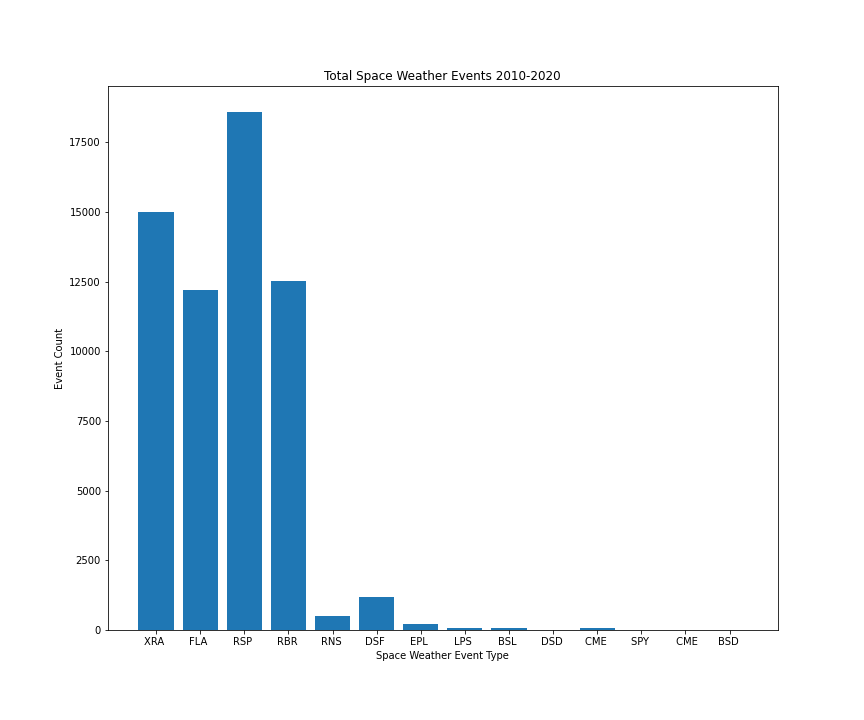
\includegraphics[width=12cm]{figures/Space_Weather_Plot.png}
    \centering
    \caption{Total number of space weather events observed since 2010, grouped by event type (Event types are listed in table \ref{space_weather_events})}
    \label{swe_freq}
\end{figure}

\begin{table}
\centering
\caption*{AIA Filter Summary}
\begin{tabular}{||c | c | c | c ||} 
 \hline
 Wavelength (\AA) & Primary Emission Source & Region of Atmosphere & log(T)\\ [0.5ex] 
 \hline\hline
  4500 & Continuum & Photosphere & 3.7 \\
 \hline
 1700 & Continuum & Photosphere & 3.7 \\
 \hline
 1600 & C IV + Continuum & Upper Photosphere / Transition Region & 4.7 \\
 \hline
 335 & Fe XVI & Flaring Regions & 6.8 \\
 \hline
 304 & He II & Chromosphere / Transition Region & 5.8 \\
 \hline
 211 & Fe XIV & Active-Region Corona & 6.3 \\
 \hline
 193 & Fe XII, XXIV & Corona and Hot Flare Plasma & 6.1, 7.3 \\
 \hline 
 171 & Fe IX & Quiet Corona / Upper Transition Region & 5.0 \\
 \hline
 131 & Fe VIII, XX, XXIII & Flaring Regions & 5.6,7.0,7.2 \\
 \hline
 94 & Fe XVIII & Flaring Regions & 6.8 \\
 \hline
 
\end{tabular}
\caption{The wavelengths observed by the AIA, along with the primary source of emission at each wavelength, and the approximate location and temperature of the portion of the Sun that each wavelength probes. \cite{AIA_ConceptReport}}
\label{AIA_wavelengths}
\end{table}

\subsection*{Data Storage Concerns}
Every event has a listed start time and end time, among other parameters. We will use these start time and end time values to identify when different events should be present, and use those time frames to select the images that will make up our neural net training and testing data sets. Each single .fits file is about 10MB in size, so we will need to be selective about how many images we store. The mean duration for the four most common types of events (XRA, FLA, RBR, and RSP) since 2010 are 20, 18.5, 3.75, and 48 minutes respectively. Considering the average duration of each event, the number of total number events since the AIA began observations, and the frequency of AIA observations, we would need almost a petabyte of storage to store every image in every wavelength for which a space weather event is occurring. Focusing instead on only 5-6 filters, and using one image per event, could drop our storage needs down to about one terabyte per event type.

\section*{Background Information}

Solar flares are highly energetic events of localized increased brightness on the sun over a time period ranging from milliseconds to over an hour. This brightness can be seen across many wavelengths, including x-ray, optical, and radio, and can be seen in Figure \ref{flare}. They tend to be associated with groups of sunspots — localized regions of cooler material and strong magnetic fields — and are often accompanied by the ejection of charged particles. These particles, as well as high-energy electromagnetic radiation, can affect electrical systems and the Earth’s ionosphere, and have the potential to cause major disruptions \cite{BOB}. The main goal of the Solar Dynamics Observatory is to understand the mechanisms of these events which have the potential of affecting life on Earth \cite{Pesnell2012}. The precise cause of solar flares remains uncertain, but a leading theory is that energy is suddenly released from the strong magnetic field in sunspots through a process called reconnection. This occurs when a magnetic field loop ``breaks" and ``reconnects" in a more stable path, releasing most of the energy stored in the loop \cite{BOB}. An additional process which appears in our images is granulation, which occurs as a result of convection in the solar atmosphere. Granules tend to span around 700~km and have lifetimes of five to ten minutes \cite{BOB}. Since we are analyzing how the Sun is changing over time, the granulation pattern can show up in our images, as seen in Figure \ref{flare_diff}.

There are some successful prior efforts to predict the solar flares based on changes in the Sun’s magnetic field \cite{Raboonik2016}; however, because solar flare events are associated with changes in the Sun’s magnetic field, it may not be possible to directly predict them through purely visual means. Should our prediction method turn out to be satisfactory, it would provide an unprecedented view about the nature of solar flares that the solar flares are correlated to the dynamics of the sun's surface in a way that we can use the emission from the sun's surface to detect and predict a solar flare.


\section*{Potential Risks}

Although the data for this project is easy to access, the biggest risk is the failure to identify events from the images we have. If machine learning on the dataset we intend to use is not capable of detecting events, there is little hope for it to be able to predict them. There are curated datasets available which improve the quality of the images in some ways; however these are made available a week after the images are taken at the earliest, and would offer little use in trying to predict events in real time \cite{Galvez2019}. In the event that the lower-quality images are unable to detect events, the curated datasets could still be useful in determining whether flare events are associated with visual changes in the Sun, which is valuable information regardless of whether it can be used to predict flares in real time.


\bibliographystyle{unsrt}
\bibliography{bibfile}
\pagebreak
\section*{Appendix}


\begin{figure}[h]
    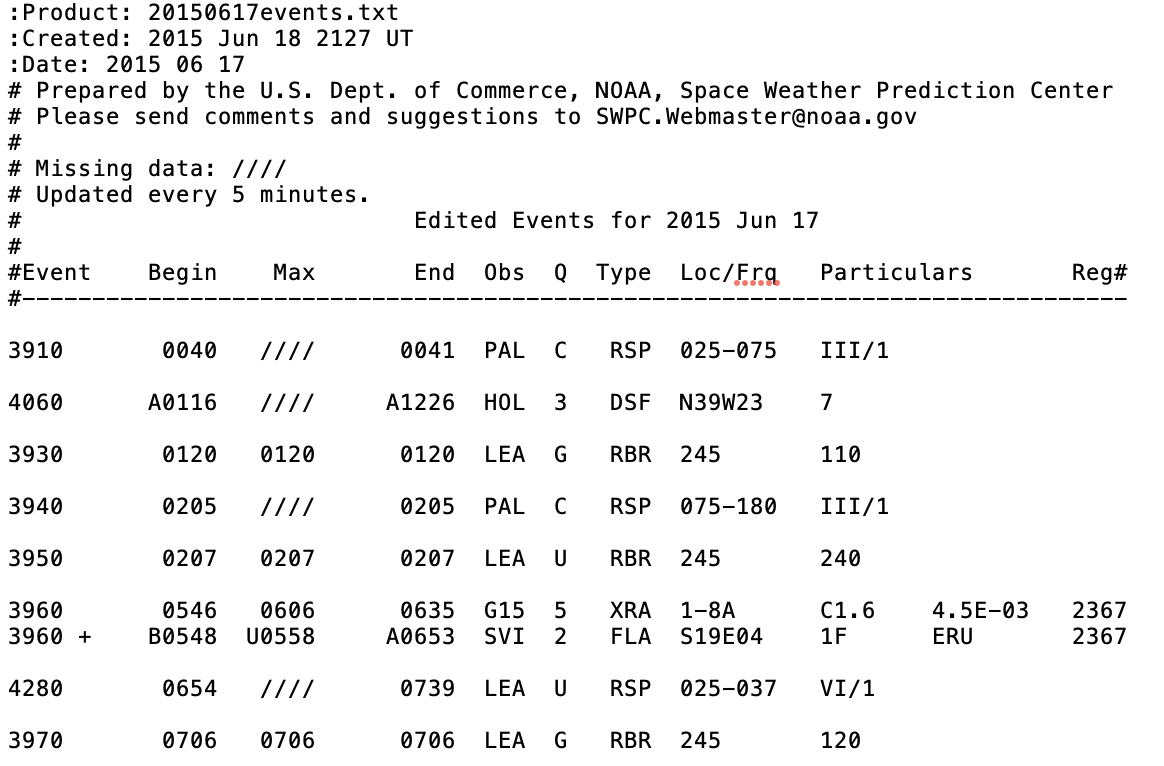
\includegraphics[width=12cm]{figures/swr_sample.png}
    \centering
    \caption{Sample Space Weather Report text file From June 6, 2015. Along with event types and times, the reports also contain information about the event strengths and locations.}
    \label{swr_sample}
\end{figure}

\begin{figure}[h]
	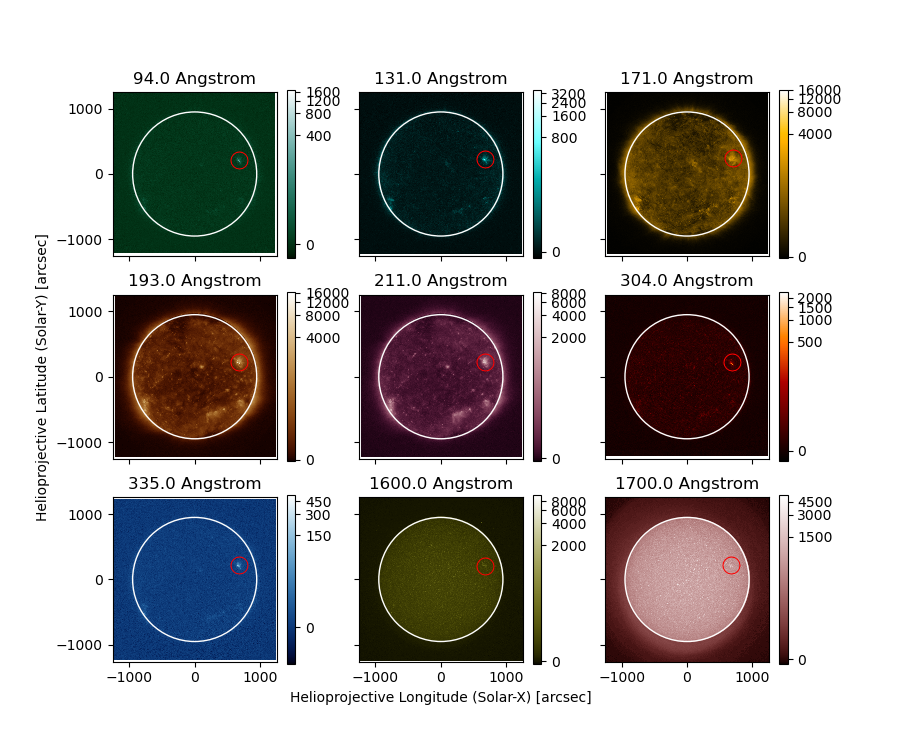
\includegraphics[width=7in]{figures/0819_flare_labeled.png}
	\centering
	\caption{A small x-ray flare which occurred August 19, 2020 in each AIA wavelength apart from 4500~\AA{}. The flare, circled in red on each image, shows up in all wavelengths to varying degrees.}
	\label{flare}
\end{figure}

\begin{figure}[h]
	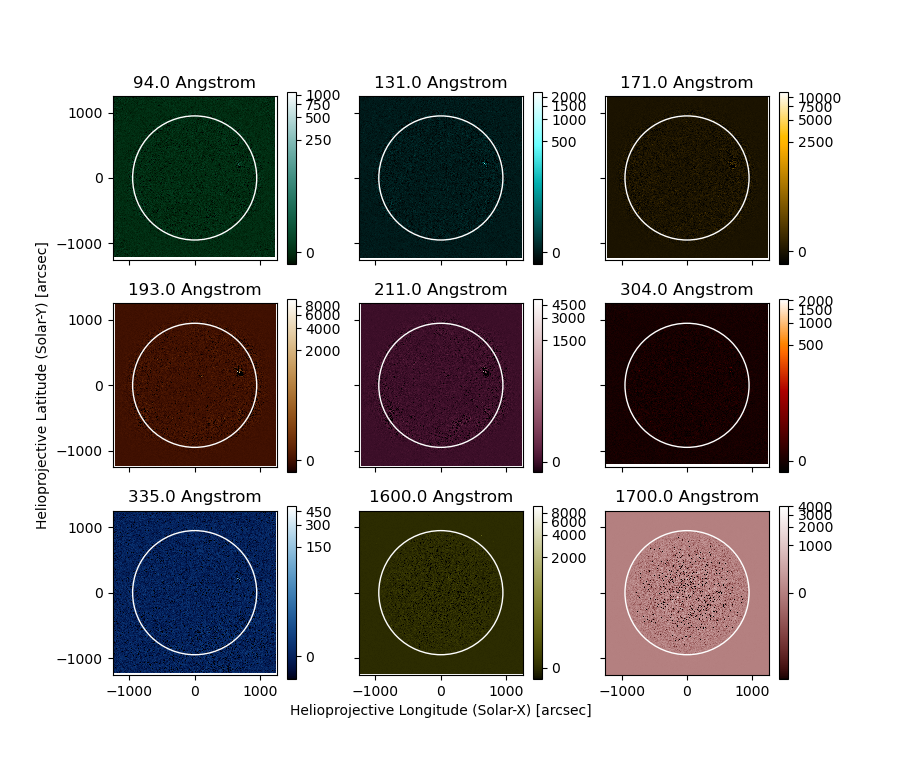
\includegraphics[width=7in]{figures/0819_flare_diff.png}
	\centering
	\caption{The same flare as above, after subtracting a previous image from the current one. This process is sometimes called difference imaging, and is useful in seeing how an object changes over time, such as the appearance of a flare. These difference images were taken over a span of two minutes, but varying this time could optimize our detection process. The changing granulation pattern is especially apparent in the 1700~\AA{} image.}
	\label{flare_diff}
\end{figure}


\end{document}
